\section{Service Discovery}
In the first section of this paper demonstrated how to containerised services in a messaging system. However, in order for the sending and receiving containers to communicate with the RabbitMQ container they need to have the IP address of the RabbitMQ container hard coded. This does not provide great flexibility. For example, autoscaling the RabbitMQ service cannot be achieved with this setup as other containers won't know the IP address of the new containers created through scaling. This creates the need for service discovery. Service discovery manages the communication of distributed service in a micro-service architecture. The service discovery tool used in this exercise is Consul.

\subsection{Setting up the System}
The system for this exercise consisted of three services running on a single ECS instance: A weather service for reporting weather details, a stock-price service for reporting stock prices and a portal which acts as a fronted for the aforementioned services. Therefore, the portal needs a way of communication with the weather and stock-price containers. Source code for these services was obtained from Github.

To create the system an ECS cluster is first created. The remaining architecture was created using a CloudFormation template obtained with the services course code and a small number of parameters, including a VPC, a subnet and Amazon DNS IP.

The Amazon DNS is a DNS server created by default in a VPC to allows instance within the VPC to talk to the VPC's Internet gateway. The IP address server can be accessed by subnest of the VPC at the network address of the subnet plus two i.e. if the subnet address is 172.31.0.0/16 then the Amazon DNS IP is 172.31.0.2. Therefore, when inserting the parameters for the CloudFormation stack it is important to ensure the subnet enter is contained within the VPC entered and that the DNS IP is the address of for that subnet.

Once the stack created and 2 EC2 instances are created. One contains the Consul Server and the other is an ECS instance which has been added to the cluster created earlier. The ECS instance is where the service will run in containers. On creation it is running a containing with a Consul agent. It is the agent that provides the service discovery mechanism to the other containers, e.g. it will allows the portal to discover and hence make requests to the weather and stock-price services.

The services were built by logging onto the Consul server instance, cloning the source code and then building images using Dockerfiles. The images where then pushed to Docker Hub.

Finally, a task definition and a service to run each image once the ECS instance was created, similar to the ECS section of this report. However, this time the ALB and Application Autoscaling policies were omitted, instead just selecting a desired number of tasks as one, for each service.

\begin{figure}[H]
	\setlength{\belowcaptionskip}{15pt plus 3pt minus 2pt}
	\caption{Portal}
	\centering
	%\includegraphics[width=\textwidth,height=\textheight,keepaspectratio]{diagram}
	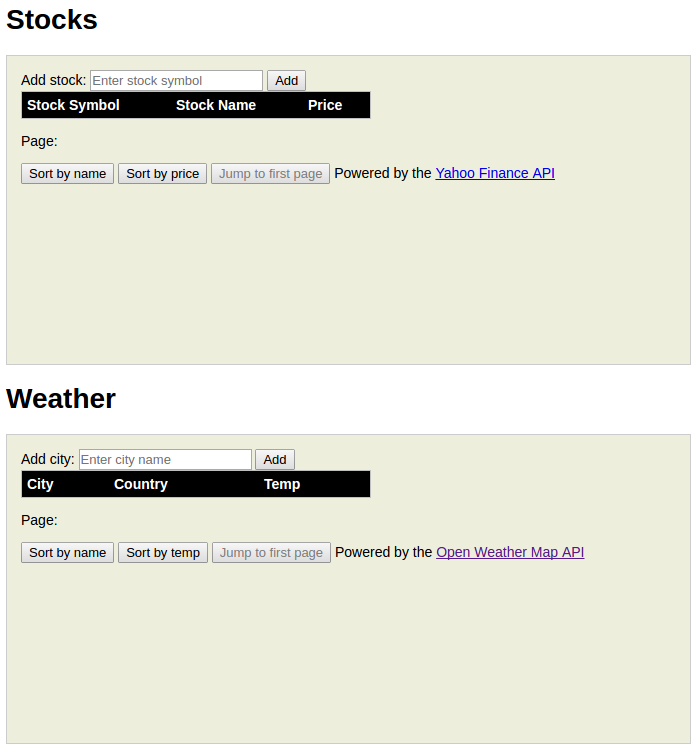
\includegraphics[width=\textwidth,keepaspectratio]{stocks-and-weather}
	\label{fig:rabbit}
\end{figure}